% Figure 3.3: conceptual action-centred property graph.
% Replacement for the supplied tikzpicture; requires \usepackage{tikz}.
% No additional TikZ libraries are required.
% Asset 0 and Asset 1 identify pool participants, not fixed swap directions.
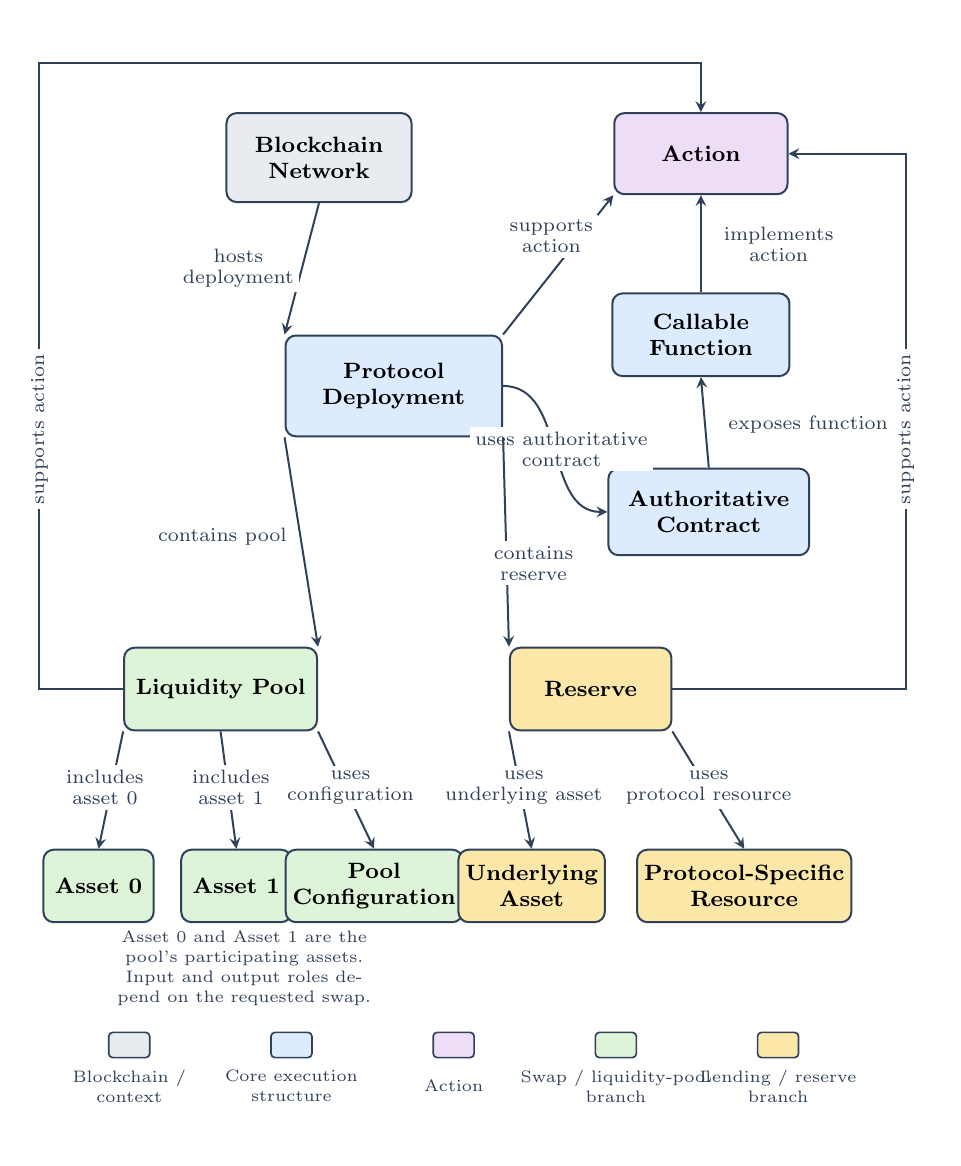
\begin{tikzpicture}[x=1cm,y=1cm,>=stealth]
\path[use as bounding box] (0,0) rectangle (11.5,14.1);

\definecolor{graphline}{HTML}{2F425A}
\definecolor{contextfill}{HTML}{E8ECF0}
\definecolor{corefill}{HTML}{DCEBFE}
\definecolor{actionfill}{HTML}{EEDDF6}
\definecolor{swapfill}{HTML}{DDF4D9}
\definecolor{lendfill}{HTML}{FBE8A9}

\tikzset{
  entity/.style={rectangle, rounded corners=0.13cm, draw=graphline,
    line width=0.72pt, align=center, text=black, inner sep=2.5pt,
    font=\fontsize{8.4}{9.4}\selectfont\bfseries},
  relation/.style={->, draw=graphline, line width=0.72pt},
  relationlabel/.style={text=graphline, align=center, fill=white,
    inner sep=1.8pt, font=\fontsize{6.8}{7.6}\selectfont},
  legendlabel/.style={text=graphline, align=center,
    font=\fontsize{6.4}{7.2}\selectfont}
}

% Core entities.
\node[entity,fill=contextfill,minimum width=2.35cm,minimum height=1.13cm]
  (network) at (3.70,12.45) {Blockchain\\Network};
\node[entity,fill=actionfill,minimum width=2.20cm,minimum height=1.03cm]
  (action) at (8.55,12.50) {Action};
\node[entity,fill=corefill,minimum width=2.75cm,minimum height=1.28cm]
  (deployment) at (4.65,9.55) {Protocol\\Deployment};
\node[entity,fill=corefill,minimum width=2.25cm,minimum height=1.05cm]
  (function) at (8.55,10.20) {Callable\\Function};
\node[entity,fill=corefill,minimum width=2.55cm,minimum height=1.10cm]
  (contract) at (8.65,7.95) {Authoritative\\Contract};

% Swap branch: separate nodes for the two participating token contracts.
\node[entity,fill=swapfill,minimum width=2.45cm,minimum height=1.05cm]
  (pool) at (2.45,5.70) {Liquidity Pool};
\node[entity,fill=swapfill,minimum width=1.40cm,minimum height=0.92cm]
  (assetZero) at (0.90,3.20) {Asset 0};
\node[entity,fill=swapfill,minimum width=1.40cm,minimum height=0.92cm]
  (assetOne) at (2.65,3.20) {Asset 1};
\node[entity,fill=swapfill,minimum width=1.70cm,minimum height=0.92cm]
  (poolConfig) at (4.40,3.20) {Pool\\Configuration};

% Lending branch.
\node[entity,fill=lendfill,minimum width=2.05cm,minimum height=1.05cm]
  (reserve) at (7.15,5.70) {Reserve};
\node[entity,fill=lendfill,minimum width=1.75cm,minimum height=0.92cm]
  (assetLend) at (6.40,3.20) {Underlying\\Asset};
\node[entity,fill=lendfill,minimum width=2.55cm,minimum height=0.92cm]
  (resource) at (9.10,3.20) {Protocol-Specific\\Resource};

% The two resource-to-action links are routed around the outside so that
% they do not cross the core execution or asset branches.
\draw[relation] (pool.west) -- (0.15,5.70) -- (0.15,13.65)
  -- (8.55,13.65) -- (action.north);
\node[relationlabel,rotate=90] at (0.15,9.00) {supports action};
\draw[relation] (reserve.east) -- (11.15,5.70) -- (11.15,12.50)
  -- (action.east);
\node[relationlabel,rotate=90] at (11.15,9.00) {supports action};

% Network and execution structure.
\draw[relation] (network.south) -- (deployment.north west);
\node[relationlabel,anchor=east] at (3.45,11.05) {hosts\\deployment};

\draw[relation] (deployment.north east) -- (action.south west);
\node[relationlabel] at (6.65,11.45) {supports\\action};

\draw[relation] (function.north) -- (action.south);
\node[relationlabel,anchor=west] at (8.77,11.35) {implements\\action};

\draw[relation] (contract.north) -- (function.south);
\node[relationlabel,anchor=west] at (8.83,9.06) {exposes function};

\draw[relation] (deployment.east) to[out=0,in=180] (contract.west);
\node[relationlabel] at (6.78,8.75) {uses authoritative\\contract};

% Deployment membership does not by itself establish action availability.
\draw[relation] (deployment.south west) -- (pool.north east);
\node[relationlabel,anchor=east] at (3.36,7.63) {contains pool};
\draw[relation] (deployment.south east) -- (reserve.north west);
\node[relationlabel,anchor=west] at (5.85,7.30) {contains\\reserve};

% Pool endpoints and configuration.
\draw[relation] (pool.south west) -- (assetZero.north);
\node[relationlabel] at (0.98,4.45) {includes\\asset 0};
\draw[relation] (pool.south) -- (assetOne.north);
\node[relationlabel] at (2.58,4.45) {includes\\asset 1};
\draw[relation] (pool.south east) -- (poolConfig.north);
\node[relationlabel] at (4.10,4.45) {uses\\configuration};

% Reserve endpoints and additional protocol resources.
\draw[relation] (reserve.south west) -- (assetLend.north);
\node[relationlabel] at (6.30,4.45) {uses\\underlying asset};
\draw[relation] (reserve.south east) -- (resource.north);
\node[relationlabel] at (8.65,4.45) {uses\\protocol resource};

% Asset roles are request-specific; they are not additional graph entities.
\node[legendlabel,text width=5.0cm] at (2.75,2.15)
  {Asset 0 and Asset 1 are the pool's participating assets.\\
   Input and output roles depend on the requested swap.};

% Legend: colours distinguish conceptual roles, not trust or approval status.
\foreach \pos/\colour in {
  1.29/contextfill,3.35/corefill,5.41/actionfill,7.47/swapfill,9.53/lendfill}{
  \draw[draw=graphline,fill=\colour,line width=0.60pt,rounded corners=0.05cm]
    (\pos-0.26,1.02) rectangle (\pos+0.26,1.34);
}
\node[legendlabel] at (1.29,0.66) {Blockchain /\\context};
\node[legendlabel] at (3.35,0.66) {Core execution\\structure};
\node[legendlabel] at (5.41,0.66) {Action};
\node[legendlabel] at (7.47,0.66) {Swap / liquidity-pool\\branch};
\node[legendlabel] at (9.53,0.66) {Lending / reserve\\branch};
\end{tikzpicture}
